% !TEX encoding = UTF-8
% !TEX TS-program = pdflatex
% !TEX root = ../relazione.tex
% !TEX spellcheck = it-IT

\clearpage
\section{Prove effettuate}

Una volta implementato il codice dei vari algoritmi e dopo aver verificato l'assenza di errori, sono state effettuate varie prove, i cui risultati vengono riportati nelle successive sotto sezioni.

C'è da osservare che nella maggior parte delle prove, gli algoritmi presi in cosiderazione sono stati eseguiti $1000$ volte, pertanto il rapporto $\frac{\text{\# sol. ottime}}{\text{\# esecuzioni}}$ rappresenta una stima della probabilità di trovare la soluzione ottima per un determinato problema e questa stima risulta essere sempre meno accurata al crescere della dimensione del problema.

Di conseguenza la stima della probabilità di trovare una soluzione ottima per $4$-Regine risulta molto più accurata della stima per $10$-Regine, questo a casua della crescita esponziale del numero degli stati del problema.

\subsection{Confronto tra i vari algoritmi}

La prima prova effettuata è stata l'esecuzione di Hill Climbing, Hill Climbing con mosse laterali e Hill Climbing stocastico per risolvere $N$-Regine a partire da $4$-Regine fino a $25$-regine.

Ognuno dei problemi è stato risolto sia a partire da uno stato iniziale fisso, ovvero con tutte le regine nella prima riga, sia da uno stato generato casualmente. Inoltre, per ognuno di questi casi sono state effettuate $1000$ esecuzioni di ogni algoritmo.

Dai risultati ottenuti, riportati nelle tabelle \ref{table:allinitial} e \ref{table:allrandom}, si può osservare che:

\begin{itemize}

\item Hill Climbing laterale riesce quasi sempre a trovare una soluzione ottima, mentre le Hill Climbing normale e stocastico fanno sempre più fatica a raggiungere l'ottimo.

\item Hill Climbing stocastico non migliora di molto l'Hill Climbing normale, solamente in alcuni casi trova più soluzioni ottime richiedendo più mosse. Tuttavia, uno dei vantaggi della versione stocastica di Hill Climbing è quello che dovrebbe trovare soluzioni migliori e la prova effettuata non tiene conto della qualità delle soluzioni sub-ottime. Pertanto è stata effettuata un'altra prova tenendo conto anche di questo. Tale prova è descritta nella sezione §\ref{prove:stocastico}.

\item Hill Climbing riesce sempre a trovare a trovare una soluzione a 4-regine partendo dallo stato inizile fisso in 3 mosse. Questo perché, le azioni possibili per la prima mossa sono \texttt{(1,3)} oppure \texttt{(2,3)} e una caratteristica delle soluzioni ottime di 4-Regine è di avere la forma \texttt{<X,0,3,X>} o \texttt{<X,3,0,X>}. Partendo da uno stato casuale invece non sempre viene scelta una di queste mosse, arrivando così a delle soluzioni sub-ottime. 

\item Il problema 6-Regine risulta essere particolarmente difficile da risolvere, sia a partire da uno stato fisso che da uno stato casuale. \`{E} stato quindi affrontato più nel dettaglio applicando solamente Hill Climbing laterale dal momento che è l'algoritmo che sta dando i risultati migliori. La descrizione di questa prova è nella sezione §{prove:6regine}.
\end{itemize}

\begin{table}[]
\centering
\resizebox{\textwidth}{!}{%
\begin{tabular}{|c|c|c|c|c|c|c|c|c|c|}
\hline
   & \multicolumn{3}{c|}{Hill Climbing} & \multicolumn{3}{c|}{Hill Climbing laterale} & \multicolumn{3}{c|}{Hill Climbing stocastico} \\ \hline
N  & Tempo (s)  & Mosse  & Sol. Ottime  & Tempo (ms)     & Mosse     & Sol. Ottime    & Tempo (s)      & Mosse      & Sol. Ottime     \\ \hline
4                      & 0,00049    & 3      & 1000         & 0,00049        & 3         & 1000           & 0,00058        & 3,29       & 526             \\ \hline
5                      & 0,00120    & 3,95   & 793          & 0,00130        & 4,57      & 1000           & 0,00149        & 4,88       & 715             \\ \hline
6                      & 0,00259    & 4,52   & 213          & 0,02017        & 41,81     & 888            & 0,00335        & 6          & 116             \\ \hline
7                      & 0,00464    & 5,54   & 415          & 0,01280        & 16,44     & 946            & 0,00645        & 7,51       & 264             \\ \hline
8                      & 0,00829    & 6,44   & 184          & 0,02982        & 25,50     & 930            & 0,01200        & 9,10       & 158             \\ \hline
9                      & 0,01367    & 7,48   & 223          & 0,04485        & 25,34     & 943            & 0,02043        & 10,64      & 106             \\ \hline
10                     & 0,02197    & 8,47   & 119          & 0,09734        & 39,73     & 892            & 0,03408        & 12,26      & 69              \\ \hline
11                     & 0,03326    & 9,41   & 78           & 0,13012        & 38,87     & 916            & 0,05385        & 13,82      & 42              \\ \hline
12                     & 0,05009    & 10,41  & 74           & 0,17047        & 37,35     & 952            & 0,08068        & 15,31      & 34              \\ \hline
13                     & 0,07175    & 11,39  & 48           & 0,22080        & 36,75     & 962            & 0,11831        & 17,04      & 38              \\ \hline
14                     & 0,10134    & 12,46  & 53           & 0,29341        & 37,64     & 975            & 0,16871        & 18,68      & 43              \\ \hline
15                     & 0,13929    & 13,42  & 45           & 0,37876        & 37,70     & 971            & 0,23528        & 20,38      & 27              \\ \hline
16                     & 0,19675    & 14,15  & 40           & 0,49206        & 38,20     & 978            & 0,32068        & 21,96      & 33              \\ \hline
17                     & 0,26655    & 15,50  & 38           & 0,62832        & 39,02     & 988            & 0,43232        & 23,66      & 26              \\ \hline
18                     & 0,32632    & 16,49  & 25           & 0,79175        & 39,93     & 984            & 0,57571        & 25,54      & 24              \\ \hline
19                     & 0,42260    & 17,50  & 27           & 0,99589        & 41,24     & 983            & 0,74080        & 26,97      & 20              \\ \hline
20                     & 0,53441    & 18,51  & 25           & 1,21197        & 41,56     & 995            & 0,95826        & 28,85      & 22              \\ \hline
21                     & 0,67142    & 19,49  & 13           & 1,47746        & 42,32     & 993            & 1,21045        & 30,40      & 17              \\ \hline
22                     & 0,84227    & 20,60  & 21           & 1,76070        & 42,49     & 998            & 1,51940        & 32,06      & 13              \\ \hline
23                     & 1,03802    & 21,57  & 23           & 2,08641        & 43,27     & 996            & 1,89762        & 33,92      & 13              \\ \hline
24                     & 1,27302    & 22,56  & 20           & 2,55409        & 43,27     & 997            & 2,32966        & 33,50      & 13              \\ \hline
25                     & 1,56128    & 23,60  & 24           & 2,96620        & 45,52     & 998            & 2,83871        & 37,12      & 10              \\ \hline
\end{tabular}
}
\caption{Risultati medi di 1000 esecuzioni dei vari algoritmi a partire da uno stato iniziale fisso.}
\label{table:allinitial}
\end{table}
\begin{table}[]
\centering
\resizebox{\textwidth}{!}{%
\begin{tabular}{|c|c|c|c|c|c|c|c|c|c|}
\hline
   & \multicolumn{3}{c|}{Hill Climbing} & \multicolumn{3}{c|}{Hill Climbing laterale} & \multicolumn{3}{c|}{Hill Climbing stocastico} \\ \hline
N  & Tempo (s)  & Mosse  & Sol. Ottime  & Tempo (ms)     & Mosse     & Sol. Ottime    & Tempo (s)      & Mosse      & Sol. Ottime     \\ \hline
4  & 0,00034    & 1,56   & 428          & 0,00041        & 2,86      & 1000           & 0,00035        & 1,82       & 341             \\ \hline
5  & 0,00074    & 2,14   & 690          & 0,00084        & 3,03      & 1000           & 0,00081        & 2,72       & 693             \\ \hline
6  & 0,00158    & 2,30   & 121          & 0,01276        & 45,93     & 814            & 0,00178        & 3,01       & 87              \\ \hline
7  & 0,00273    & 2,82   & 276          & 0,00864        & 15,65     & 912            & 0,00323        & 3,81       & 250             \\ \hline
8  & 0,00476    & 3,20   & 123          & 0,01836        & 22,71     & 930            & 0,00571        & 4,45       & 112             \\ \hline
9  & 0,00791    & 3,65   & 154          & 0,02660        & 22,66     & 924            & 0,00978        & 5,19       & 168             \\ \hline
10 & 0,01218    & 4,96   & 54           & 0,06255        & 39,36     & 860            & 0,01561        & 5,73       & 52              \\ \hline
11 & 0,01849    & 4,43   & 41           & 0,09029        & 38,86     & 897            & 0,02436        & 6,41       & 47              \\ \hline
12 & 0,02783    & 4,82   & 44           & 0,11035        & 34,62     & 930            & 0,03590        & 7,09       & 54              \\ \hline
13 & 0,039987   & 5,29   & 25           & 0,15324        & 32,77     & 968            & 0,05288        & 7,85       & 36              \\ \hline
14 & 0,05579    & 5,71   & 24           & 0,19152        & 32,68     & 964            & 0,07559        & 8,60       & 36              \\ \hline
15 & 0,07528    & 6,20   & 43           & 0,26458        & 31,88     & 969            & 0,10317        & 9,22       & 29              \\ \hline
16 & 0,10097    & 6,71   & 24           & 0,31388        & 30,47     & 987            & 0,13739        & 10,09      & 24              \\ \hline
17 & 0,13565    & 7      & 30           & 0,42151        & 33,20     & 980            & 0,18781        & 10,69      & 24              \\ \hline
18 & 0,17606    & 7,56   & 24           & 0,50562        & 31,41     & 984            & 0,24386        & 11,39      & 15              \\ \hline
19 & 0,22452    & 7,86   & 18           & 0,64227        & 31,63     & 993            & 0,31848        & 12,19      & 16              \\ \hline
20 & 0,28445    & 8,31   & 26           & 0,76014        & 31,75     & 989            & 0,40667        & 12,91      & 20              \\ \hline
21 & 0,35974    & 8,81   & 13           & 0,93101        & 33,32     & 992            & 0,51567        & 13,55      & 17              \\ \hline
22 & 0,44227    & 9,25   & 15           & 1,11264        & 33,58     & 994            & 0,64465        & 14,29      & 17              \\ \hline
23 & 0,52948    & 9,71   & 11           & 1,31210        & 32,51     & 991            & 0,80020        & 14,98      & 11              \\ \hline
24 & 0,66810    & 10,31  & 9            & 1,58736        & 32,82     & 996            & 0,98633        & 15,80      & 12              \\ \hline
25 & 0,81686    & 10,53  & 9            & 1,85988        & 33,77     & 999            & 1,20711        & 16,68      & 16              \\ \hline
\end{tabular}
}
\caption{Risultati medi di 1000 esecuzioni dei vari algoritmi a partire da uno stato iniziale generato casualmente.}
\label{table:allrandom}
\end{table}

\subsection{Riavvi casuali}

In questa prova sono state eseguite le precedenti versioni di Hill Climbing utilizzando però la versione a riavvio casuale.

Anche in questo caso i problemi risolti vanno da $4$-Regine a $25$-Regine, ognuno risolto $100$ volte, sia a partire dallo stato iniziale con tutte le regine su una stessa riga, che a partire da uno stato generato casualmente.

A differenza della prova precedente, sono stati presi in considerazioni i riavvii necessari per trovare una soluzione ottima piuttosto del numero delle mosse per ottenere una soluzione ottima.

Così facendo è stato possibile verificare che il numero medio di riavvii coincida con quanto atteso, ovvero $\frac{1}{p}$, dove $p$ è la probabilità di trovare una soluzione ottima.

I risultati ottenuti sono riportati nella tabella \ref{table:riavvii} e la differenza dei valori ottenuti da quelli attesi viene evidenziata nella nel grafico della figura \ref{fig:riavvii}.

Dal grafico si può notare che la maggior parte dei risultati non si discosta di molto, ci sono solamente alcuni casi in cui la differenza è notevole e questo può essere causato dal numero ridotto di prove effettuate, che per motivi di tempo sono state limitate a 100.
In ogni caso, la differenza media risulta essere inferiore al $20\%$ per Hill Climbing e poco più del $15\%$ per Hill Climbing stocastico.

% Please add the following required packages to your document preamble:
% \usepackage{graphicx}
\begin{table}[]
\centering
\resizebox{\textwidth}{!}{%
\begin{tabular}{|c|c|c|c|c|c|c|c|c|c|}
\hline
   & \multicolumn{3}{c|}{Hill Climbing}               & \multicolumn{3}{c|}{Hill Climbing laterale (100 mosse)} & \multicolumn{3}{c|}{Hill Climbing stocastico}   \\ \hline
N  & Media Riavvii & Riavvii attesi & Differenza (\%) & Media Riavvii    & Riavvii attesi   & Differenza (\%)   & Media Riavvii & Riavvii attesi & Differenza(\%) \\ \hline
4  & 1             & 2,34           & 57,20           & 1                & 1                & 0                 & 2,14          & 2,93           & 27,03          \\ \hline
5  & 1,22          & 1,45           & 15,82           & 1                & 1                & 0                 & 1,44          & 1,44           & 0,21           \\ \hline
6  & 8,22          & 8,26           & 0,54            & 1,15             & 1,23             & 6,39              & 8,20          & 11,49          & 28,66          \\ \hline
7  & 3,15          & 3,62           & 13,06           & 1,07             & 1,19             & 2,42              & 3,76          & 4              & 6              \\ \hline
8  & 7,15          & 8,13           & 12,06           & 1,07             & 1,08             & 0,49              & 7,68          & 8,93           & 13,98          \\ \hline
9  & 5,90          & 6,49           & 9,14            & 1,02             & 1,08             & 5,75              & 7,65          & 5,95           & 28,52          \\ \hline
10 & 16,88         & 18,52          & 8,85            & 1,14             & 1,16             & 1,96              & 16,31         & 19,23          & 15,19          \\ \hline
11 & 18,87         & 24,39          & 22,63           & 1,11             & 1,11             & 0,43              & 20,64         & 21,28          & 2,99           \\ \hline
12 & 18,60         & 22,73          & 18,16           & 1,06             & 1,08             & 1,42              & 24,77         & 18,52          & 33,76          \\ \hline
13 & 24,10         & 28.57          & 15,65           & 1,07             & 1,03             & 3,58              & 25,15         & 27,78          & 9,46           \\ \hline
14 & 32,57         & 42,67          & 21,83           & 1,06             & 1,04             & 2,18              & 28,89         & 27,78          & 4              \\ \hline
15 & 28,84         & 23,26          & 24,01           & 1,02             & 1,03             & 1,16              & 34,55         & 34,48          & 0,20           \\ \hline
16 & 45,11         & 41,67          & 8,26            & 1,03             & 1,01             & 1,66              & 38,55         & 41,67          & 7,48           \\ \hline
17 & 43,61         & 33,33          & 30,83           & 1,02             & 1,02             & 0,04              & 48,29         & 41,67          & 7,48           \\ \hline
18 & 53,33         & 41,67          & 22,99           & 1,02             & 1,02             & 0,37              & 51,20         & 66,67          & 23,20          \\ \hline
19 & 46,83         & 55,56          & 15,71           & 1,01             & 1,01             & 0,29              & 53,07         & 62,50          & 15,09          \\ \hline
20 & 51,86         & 38,46          & 34,84           & 1                & 1,01             & 1,10              & 61,56         & 50             & 23,12          \\ \hline
21 & 61,48         & 76,92          & 20,08           & 1,02             & 1,01             & 1,18              & 53,35         & 58,82          & 9,30           \\ \hline
22 & 67,62         & 66,67          & 1,43            & 1                & 1,01             & 0,60              & 60,67         & 58,82          & 3,14           \\ \hline
23 & 66,27         & 90,91          & 27,10           & 1                & 1,01             & 0,90              & 69,21         & 90,91          & 23,87          \\ \hline
24 & 86,88         & 111,11         & 21,81           & 1                & 1,01             & 0,40              & 70,11         & 83,33          & 15,87          \\ \hline
25 & 90,62         & 111,11         & 18,44           & 1,03             & 1                & 2,90              & 78,64         & 62,50          & 25,82          \\ \hline
\end{tabular}
}
\caption{Risultati medi di 100 esecuzioni dell'Hill Climbing con riavvii casuali, utilizzando le varie versioni di Hill Climbing. Alcune differenze espresse in \% sono diverse da quelle attese, questo perché la tabella riporta i risultati approssimati e le differenze sono state calcolate utilizzando i dati non approssimati.}
\label{table:riavvii}
\end{table}

\begin{figure}[ht]
\centering
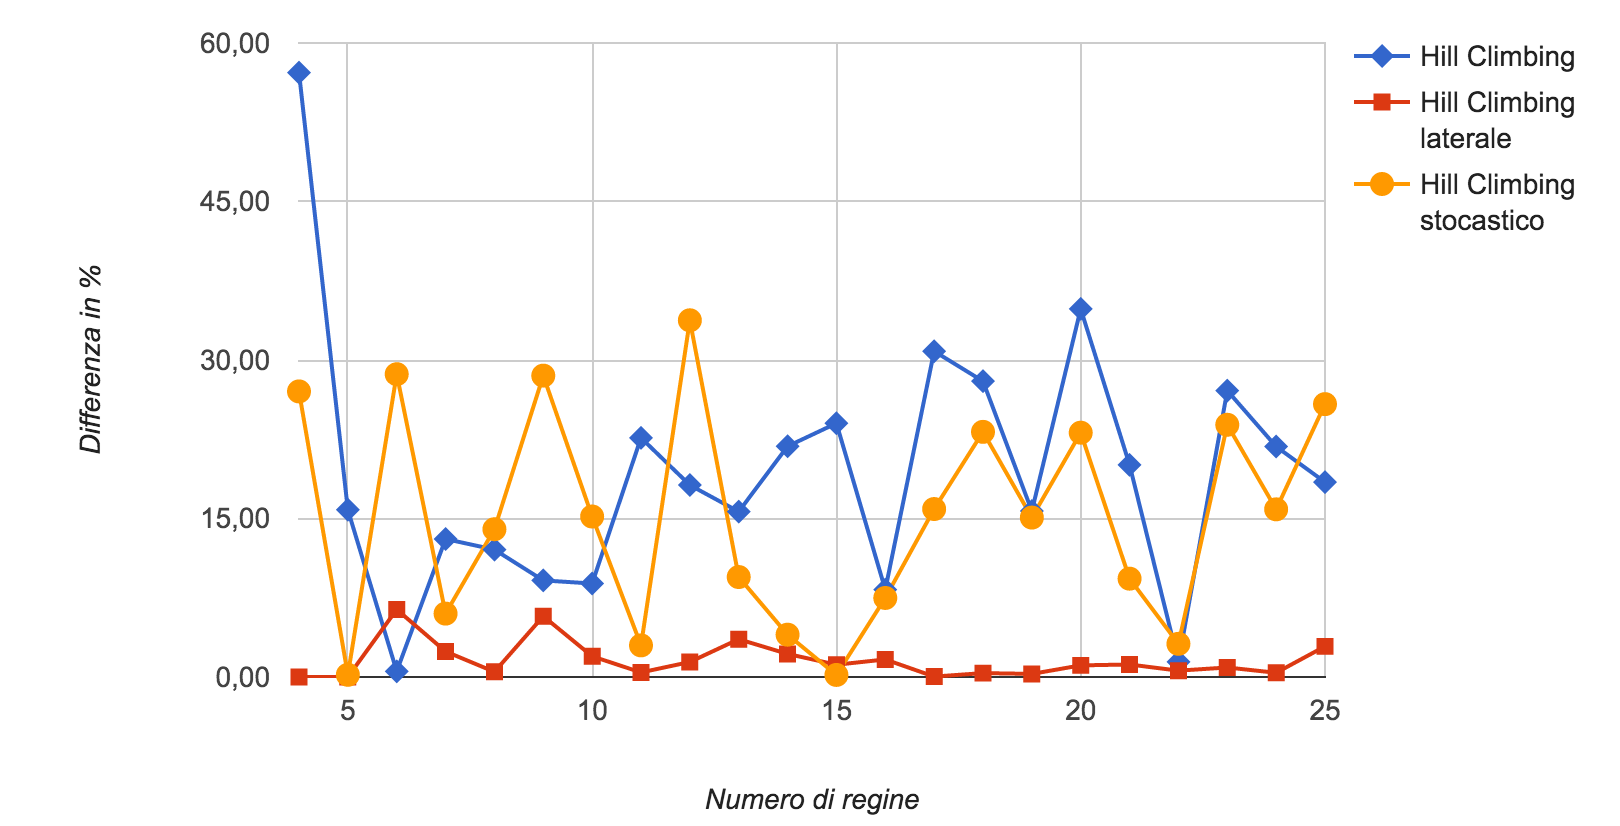
\includegraphics[width=\textwidth]{./immagini/diff-riavvii.png}
\caption{Valore assoluto della differenza tra il numero di riavvi attesi e quello medio, espresso in percentuale.}
\label{fig:riavvii}
\end{figure}

\FloatBarrier
\subsection{8-Regine}\label{prove:8regine}

La prima volta che sono state eseguite le varie versioni di Hill Climbing per risolvere il problema delle $8$-Regine, è risultata una probabilità di trovare una soluzione ottima molto più elevata di quella riportata sul libro del corso.
In particolare, stando a quanto riportato, la probabilità di trovare una soluzione ottima con Hill Climbing a partire da uno stato casuale è del $14\%$, mentre alla prima esecuzione è stata stimata essere del $28\%$ .

\`{E} stato quindi ricontrollato il codice prodotto è stato scoperto un errore nella funzione che genera gli stati del problema in modo casuale, la quale ogni tanto generava degli stati inziali con una regina posizionata fuori dalla scacchiera. 
Ad esempio nel caso delle $8$-Regine potevano venir prodotti degli stati iniziali con una regina nella riga $8$ anche se la scacchiera aveva solamente le righe da $0$ a $7$.
Il problema che veniva risolto era quindi più facile e pertanto la probabilità di ottenere una soluzione ottima risultava più elevata.

Una volta corretto l'errore è stato rieseguito l'algoritmo per risolvere $100.000$ volte $8$-Regine in modo da poter controllare che fosse effettivamente quello il problema e, come si può notare dalla tabella \ref{table:8regine}, i risultati ottenuti si avvicinano molto ai risultati attesi.

L'errore nella generazione degli stati casuali ha influenzato anche i risultati di altre prove, le quali sono state ri-eseguite in modo da ottenere dei valori correttti. I risultati presenti nelle varie tabelle di questa relazione sono quelli ottenuti con la versione corretta del codice.

\begin{table}[]
\centering
\resizebox{\textwidth}{!}{%
\begin{tabular}{|l|r|r|r|}
\hline
\multicolumn{4}{|c|}{Hill Climbing} \\ \hline
 & \multicolumn{1}{c|}{Probabilità sol. ottima} & \multicolumn{1}{c|}{Mosse caso ottimo} & \multicolumn{1}{c|}{Mosse caso sub-ottimo} \\ \hline
Versione errata & 28,19\% & 3,76 & 2,87 \\ \hline
Versione corretta & 13,9\% & 4,07 & 3,06 \\ \hline
Valori attesi & 14\% & 4 & 3 \\ \hline
\multicolumn{4}{|c|}{Hill Climbing con mosse laterali (100)} \\ \hline
& \multicolumn{1}{c|}{Probabilità sol. ottima} & \multicolumn{1}{c|}{Mosse caso ottimo} & \multicolumn{1}{c|}{Mosse caso sub-ottimo} \\ \hline
Versione errata & 96,92\% & 13,39 & 70,90 \\ \hline
Versione corretta & 94,3\% & 19,06 & 61,26 \\ \hline
Valori attesi & 94\% & 21 & 64 \\ \hline
\end{tabular}
}
\caption{8-Regine: confronto tra i dati errati, quelli corretti e quelli attesi.}
\label{table:8regine}
\end{table}

\FloatBarrier
\subsection{Hill Climbing Stocastico}\label{prove:stocastico}

Dal momento che nella prima prova effettuata l'algoritmo Hill Climbing Stocastico si è rilevato meno performante dell'Hill-Climbing classico, sia in termini di tempo di esecuzione, che in numero di soluzioni ottime trovate. \`{E} stata eseguita un'ulteriore prova per verificare se le soluzioni sub-ottime trovate dalla versione stocastica siano  migliori delle soluzioni sub-ottime trovate dalla versione classica.

I risultati ottenuti sono riportati nella tabella \ref{table:stocastico} e vengono riassunti nelle figure \ref{fig:stocastico1} e \ref{fig:stocastico2}, dalle quali si può notare che:

\begin{itemize}
\item a partire da uno stato casuale, la differenza del numero delle minacce è minima;
\item a partire dallo stato con tutte le regine nella prima riga, le soluzioni sub-ottime ottenute con Hill Climbing sono migliori rispetto a quelle ottenute con la versione stocastica. 
\end{itemize}

Pertanto si può concludere che Hill Climbing Stocastico non è ideale per risolvere il problema delle N-Regine.

\begin{figure}[ht]
\centering
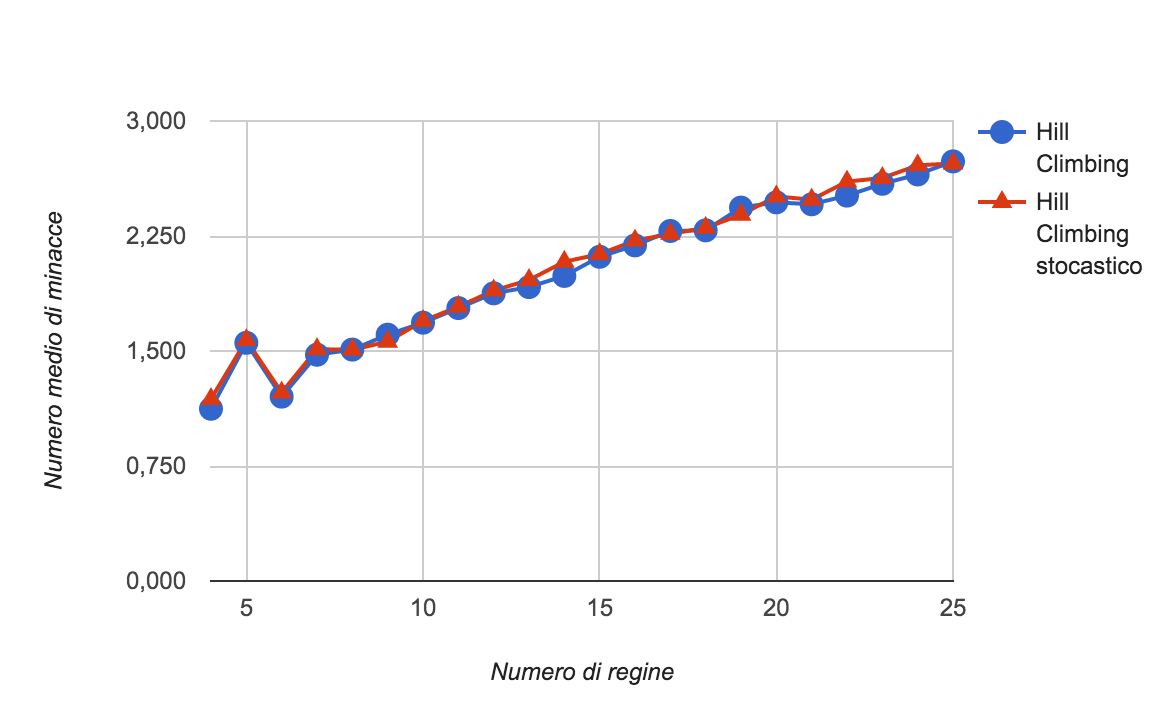
\includegraphics[width=\textwidth]{./immagini/stocastico1.png}
\caption{Differenza tra le soluzioni sub-ottime trovate con Hill Climbing e con Hill Climbing stocastico.}
\label{fig:stocastico1}
\end{figure}

\begin{figure}[ht]
\centering
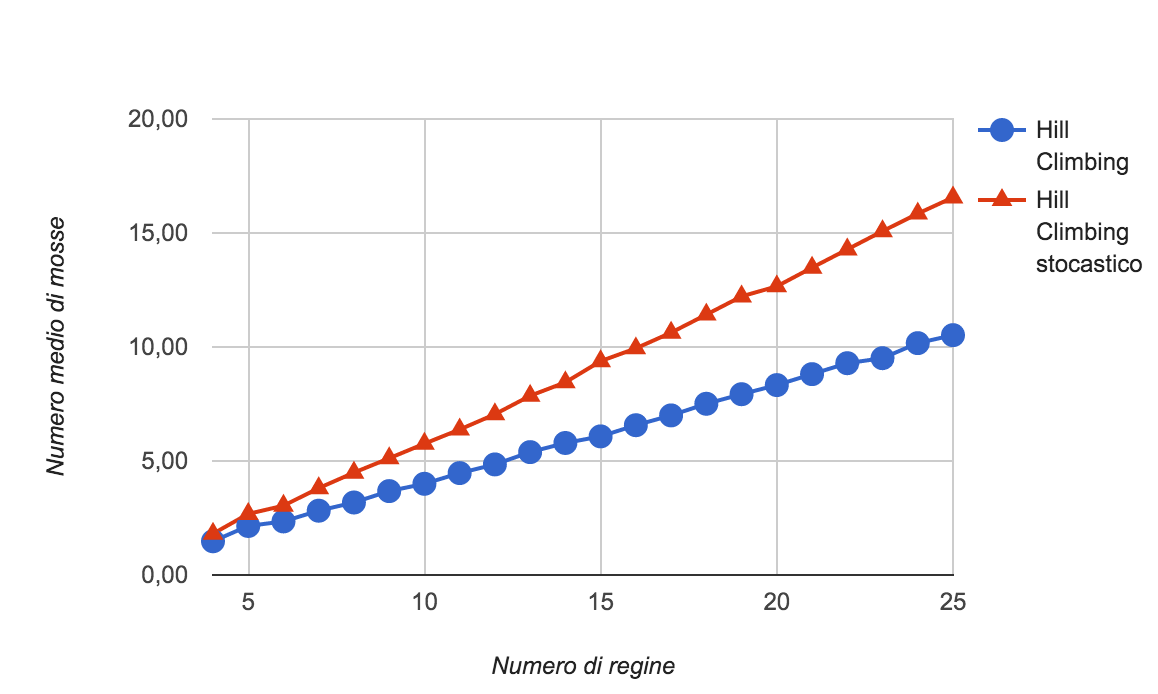
\includegraphics[width=\textwidth]{./immagini/stocastico2.png}
\caption{Numero di mosse effettaute da Hill Climbing e Hill Climbing stocatico}
\label{fig:stocastico2}
\end{figure}

% Please add the following required packages to your document preamble:
% \usepackage{graphicx}
\begin{table}[]
\centering
\resizebox{\textwidth}{!}{%
\begin{tabular}{|c|c|c|c|c|c|c|}
\hline
   & \multicolumn{3}{c|}{Hill Climbing}          & \multicolumn{3}{c|}{Hill Climbing stocastico} \\ \hline
N  & Mosse medie & Sol. Ottime & Val. Sub-ottimo & Mosse medie  & Sol. Ottime  & Val. Sub-ottimo \\ \hline
4  & 1,48        & 375         & 1,123           & 1,81         & 363          & 1,187           \\ \hline
5  & 2,15        & 709         & 1,553           & 2,68         & 692          & 1,571           \\ \hline
6  & 2,35        & 120         & 1,202           & 3,04         & 100          & 1,229           \\ \hline
7  & 2,82        & 241         & 1,476           & 3,81         & 273          & 1,512           \\ \hline
8  & 3,18        & 126         & 1,509           & 4,49         & 136          & 1,508           \\ \hline
9  & 3,68        & 129         & 1,606           & 5,12         & 132          & 1,561           \\ \hline
10 & 4           & 55          & 1,685           & 5,76         & 62           & 1,696           \\ \hline
11 & 4,47        & 41          & 1,780           & 6,38         & 46           & 1,789           \\ \hline
12 & 4,85        & 48          & 1,876           & 7,05         & 38           & 1,894           \\ \hline
13 & 5,39        & 49          & 1,917           & 7,86         & 43           & 1,963           \\ \hline
14 & 5,79        & 40          & 1,990           & 8,45         & 32           & 2,082           \\ \hline
15 & 6,08        & 21          & 2,114           & 9,38         & 33           & 2,132           \\ \hline
16 & 6,57        & 25          & 2,189           & 9,94         & 31           & 2,220           \\ \hline
17 & 7           & 31          & 2,189           & 10,63        & 16           & 2,264           \\ \hline
18 & 7,51        & 17          & 2,287           & 11,42        & 20           & 2,303           \\ \hline
19 & 7,93        & 19          & 2,435           & 12,22        & 19           & 2,389           \\ \hline
20 & 8,33        & 18          & 2,469           & 12,66        & 13           & 2,508           \\ \hline
21 & 8,81        & 15          & 2,457           & 13,48        & 6            & 2,487           \\ \hline
22 & 9,29        & 16          & 2,513           & 14,28        & 12           & 2,605           \\ \hline
23 & 9,51        & 16          & 2,590           & 15,08        & 14           & 2,628           \\ \hline
24 & 10,17       & 19          & 2,651           & 15,85        & 17           & 2,711           \\ \hline
25 & 10,52       & 14          & 2,736           & 16,56        & 19           & 2,723           \\ \hline
\end{tabular}
}
\caption{Confronto tra Hill Climbing e Hill Climbing stocastico. I risultati sono la media di 1000 prove, eseguite a partire da uno stato generato casualmente}
\label{table:stocastico}
\end{table}

\FloatBarrier
\subsection{Hill Climbing Laterale e 6-Regine}\label{prove:6regine}

Nella prima prova effettuata è emerso che Hill Climbing e le sue varianti hanno dei problemi a risolvere 6-Regine, sia a partire dallo stato iniziale che a partire da uno stato generato casualmente.

Si è quindi provato ad eseguire Hill Climbing con mosse laterali tenendo traccia del numero di mosse medie necessarie per ottenere una soluzione sub-ottima, provando a risolvere $N$-Regine con $N$ da $6$ a $9$. I risultati ottenuti sono riportati nella tabella \ref{table:6regine-lat}.

\begin{table}[]
\centering
\begin{tabular}{|c|r|r|r|}
\hline
\multicolumn{4}{|c|}{Hill Climbing Laterale (100 mosse, stato iniziale fisso)} \\ \hline
N & \multicolumn{1}{c|}{Sol. Ottime} & \multicolumn{1}{c|}{Mosse medie caso ottimo} & \multicolumn{1}{c|}{Mosse medie caso sub-ottimo} \\ \hline
6 & 881 & 34,04 & 103,86 \\ \hline
7 & 948 & 14,13 & 29,71 \\ \hline
8 & 916 & 20,74 & 100,70 \\ \hline
9 & 962 & 22,32 & 94,47 \\ \hline
\multicolumn{4}{|c|}{Hill Climbing Laterale (100 mosse, stato iniziale casuale)} \\ \hline
N & \multicolumn{1}{c|}{Sol. Ottime} & \multicolumn{1}{c|}{Mosse medie caso ottimo} & \multicolumn{1}{c|}{Mosse medie caso sub-ottimo} \\ \hline
6 & 814 & 32,66 & 101,71 \\ \hline
7 & 912 & 12,88 & 31,71 \\ \hline
8 & 930 & 18,90 & 61,49 \\ \hline
9 & 924 & 19,67 & 71,61 \\ \hline
\end{tabular}
\caption{Numero medio di mosse effettuate da Hill Climbing Laterale}
\label{table:6regine-lat}
\end{table}

Osservando il numero di mosse medie in caso di fallimento è possibile riuscire a distinguere quando l'algoritmo termina perché finisce in un minimo locale o quando termina perché finisce in un plateaux o spalla.

Infatti, se il numero medio di mosse è vicino al numero di mosse massime l'algoritmo ha terminato l'esecuzione in quanto è entrato in un plateux dal quale non è riuscito ad uscirne, mentre se il numero di mosse è inferiore al numero massimo, l'algoritmo ha terminato l'esecuzione a causa di un minimo locale, ovvero è finito in uno stato in cui tutti i suoi successori erano peggiore dello stato corrente.

Pertanto il problema che incontra HIll Climbing con $100$ mosse laterali nel risolvere $6$-Regine è causato da un plateaux che fa ciclare l'algoritmo finché non termina le mosse a disposizione.

Sono state quindi aumentate le mosse laterali a disposizione dell'algoritmo, da $100$ a $1000$, in modo da aumentare la probabilità che l'algoritmo riesca a superare il plateaux.

\begin{table}[]
\centering

\begin{tabular}{|c|c|c|c|}
\hline
\multicolumn{4}{|c|}{Hill Climbing Laterale (1000 mosse, stato iniziale fisso)} \\ \hline
N & Sol. Ottime & Mosse medie caso ottimo & Mosse medie caso sub-ottimo \\ \hline
6 & \multicolumn{1}{r|}{1000} & \multicolumn{1}{r|}{48,52} & \multicolumn{1}{r|}{0} \\ \hline
\multicolumn{4}{|c|}{Hill Climbing Laterale (1000 mosse, stato iniziale casuale)} \\ \hline
N & Sol. Ottime & Mosse medie caso ottimo & Mosse medie caso sub-ottimo \\ \hline
6 & \multicolumn{1}{r|}{937} & \multicolumn{1}{r|}{48,30} & \multicolumn{1}{r|}{1001,93} \\ \hline
\end{tabular}

\caption{Hill Climbing con $1000$ mosse laterali per risolvere $6$-Regine}
\label{table:6regine-1000}
\end{table}

Dalla tabella \ref{table:6regine-1000} si può notare che:
\begin{itemize}
\item l'algoritmo riesce sempre a trovare una soluzione ottima partendo dallo stato con tutte le regine nella prima riga, questo grazie al maggior numero di mosse laterali che gli permetto di oltrepassare dei plateaux che richiedono più di $100$ mosse;
\item il numero medio di mosse per trovare una soluzione ottima è aumentato, questo perché alcune delle soluzioni trovate dall'algoritmo richiedono più di $100$ mosse;
\item ci sono ancora dei plateaux che l'algoritmo non riesce a scavalcare e che vengono incontrati solamente partendo da uno stato casuale.
\end{itemize}

Per verificare se l'aumento delle mosse possa permettere di superare ulteriori plateux, sono stati tracciati gli stati in cui l'algoritmo si blocca perché esaurisce tutte le mosse a disposizione.

\`{E} stata così ottenuta la figura \ref{fig:ciclo} dalla quale si può vedere come l'algoritmo è rimasto incastrato in un plateaux che corrisponde ad un minimo locale, ovvero un insieme di stati tra loro raggiungibili ai quali corrisponde un minimo locale della funzione di valutazione e che hanno come vicini altri stati dell'insieme oppure stati peggiori.
In questo caso l'aumento del numero delle mosse laterali possibili non porterebbe alcuni miglioramento, in quanto l'algoritmo non ha modo di superare questa tipologia di platueax se non spostandosi su uno stato peggiore.

La maggiore difficoltà è quindi causata dalla funzione euristica utilizzata per scegliere le mosse, la quale è caratterizzata da questi minimi locali e plateux minimi che fanno terminare Hill Climbing con una soluzione sub-ottima e probabilmente l'utilizzo di un'euristica differente permette di evitare questi problemi.

In ogni caso c'è da tenere in considerazione che $6$-Regine ha solamente $4$ soluzioni mentre altri problemi più complessi come $7$ e $8$-Regine hanno rispettivamente $40$ e $92$ possibili soluzioni distinte\footnote{Questi risultati sono stati ottenuti enumerando tutte le soluzioni di $N$-Regine risolto come CSP. Maggiori informazioni sono riportate in appendice \ref{app:csp}}.

\begin{figure}[ht]
\centering
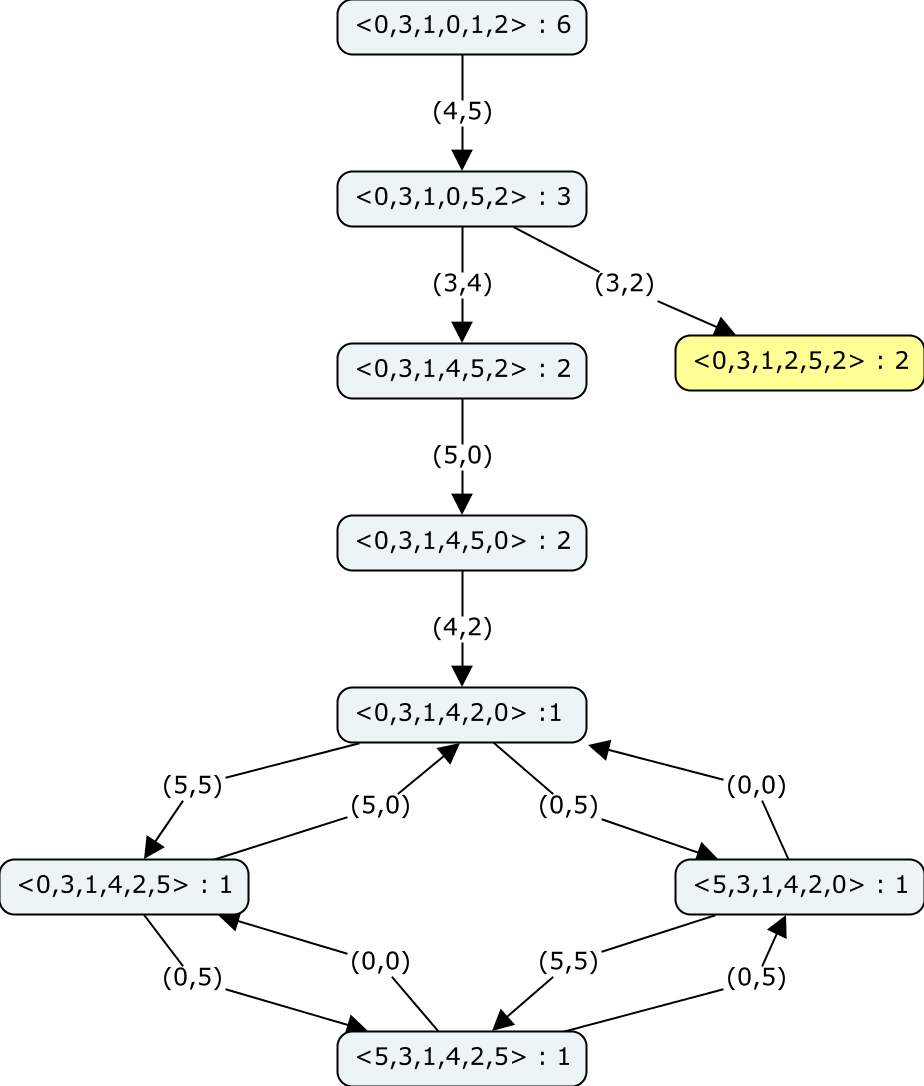
\includegraphics[width=\textwidth]{./immagini/ciclo.png}
\caption{Grafo che rappresenta gli stati visitati da Hill Climbing con $1000$ mosse laterali quando incontra un plateaux che coincide con un minimo locale. Lo stato indicato in giallo è un'alternativa che l'algoritmo \textbf{avrebbe} potuto prendere per sorpassare il primo plateaux e che forse avrebbe evitato il secondo plateux.}
\label{fig:ciclo}
\end{figure}

\FloatBarrier
\subsection{Simulated Annealing}

Come ultima prova è stato eseguito l'algoritmo Simulated Anneling per confrontare le sue prestazioni con quelle ottenute dai vari Hill Climbing.

Sono state quindi eseguite $100$ prove utilizzando come funzione di raffreddamento

\begin{align*}
temperature\_fn(t) &= 20 e^{-0,05t} \text{ se }  t < 1000 \\
&= 0  \text{ se }  t \geq 1000
\end{align*}

Dai risultati riportati nella tabella \ref{table:sa} si può osservare che l'algoritmo richiede più tempo per l'esecuzione e in alcuni casi non riesce a trovare neanche una soluzione ottima.
Questo può essere causato dal ridotto numero di prove così come dalla scelta di una funzione di raffreddamento non ottimale.

Infatti, la funzione di raffreddamento utilizzata è un variante di quella proposta dal libro di riferimento con dei parametri leggermente modificati. Questo perché la funzione proposta produce dei risultati pessimi.

Ad esempio, utilizzando la funzione $termperature\_fn(t)$ per risolvere $6$-Regine sono state ottenute $514$ soluzioni ottime su $1000$ tentativi, mentre con la funzione proposta 
dal libro, $temperature\_fn\_libro(t)$ sono state ottenute solamente $2$ soluzioni ottime.

\begin{align*}
temperature\_fn\_libro(t) &= 20 e^{-0,005t} \text{ se }  t < 100 \\
&= 0  \text{ se }  t \geq 100
\end{align*}

L'algoritmo Simulated Anneling riesce quindi ad ottenere risultati migliori di Hill Climbing e HIll Climbing stocastico, richiedendo però più tempo. 
Hill Climbing laterale risulta comunque migliore, sia in termini di soluzioni trovate che in termini di tempo d'esecuzione, anche nel problema delle $6$-Regine, dove Simulated Anneling dovrebbe essere avvantaggiato dal momento che può uscire da un plateaux minimo con una mossa peggiorativa.

% Please add the following required packages to your document preamble:
% \usepackage{graphicx}
\begin{table}[]
\centering
\resizebox{\textwidth}{!}{%
\begin{tabular}{|c|c|c|c|c|c|c|}
\hline
   & \multicolumn{3}{c|}{Simulated Annealing (stato fisso)} & \multicolumn{3}{c|}{Simulated Annealing (stato casuale)} \\ \hline
N  & Tempo (s)      & Sol. Ottime     & Val. Sub-ottimo     & Tempo (s)     & Sol. Ottime     & Val. Sub-ottimo     \\ \hline
4  & 0,08554        & 100             & 0                   & 0,08479          & 100             & 0                   \\ \hline
5  & 0,12830        & 100             & 0                   & 0,12786          & 100             & 0                   \\ \hline
6  & 0,18384        & 59              & 1                   & 0,18248          & 58              & 1                   \\ \hline
7  & 0,24730        & 79              & 1                   & 0,24532          & 76              & 1                   \\ \hline
8  & 0,32037        & 69              & 1                   & 0,31955          & 69              & 1                   \\ \hline
9  & 0,40274        & 63              & 1                   & 0,40091          & 62              & 1,03                \\ \hline
10 & 0,50208        & 28              & 1,01                & 0,49912          & 48              & 1,02                \\ \hline
11 & 0,61138        & 30              & 1,03                & 0,60908          & 32              & 1,01                \\ \hline
12 & 0,73064        & 25              & 1,09                & 0,72928          & 26              & 1,04                \\ \hline
13 & 0,86026        & 18              & 1,12                & 0,85847          & 30              & 1,14                \\ \hline
14 & 1,00010        & 15              & 1,20                & 1,00350          & 26              & 1,12                \\ \hline
15 & 1,15310        & 16              & 1,30                & 1,15272          & 14              & 1,22                \\ \hline
16 & 1,31396        & 9               & 1,31                & 1,31579          & 12              & 1,24                \\ \hline
17 & 1,62402        & 8               & 1,27                & 1,62186          & 8               & 1,30                \\ \hline
18 & 1,83081        & 10              & 1,49                & 1,82625          & 5               & 1,42                \\ \hline
19 & 2,03998        & 5               & 1,63                & 2,03762          & 8               & 1,65                \\ \hline
20 & 2,26909        & 4               & 1,69                & 2,26810          & 3               & 1,76                \\ \hline
21 & 2,50740        & 3               & 1,76                & 2,50461          & 4               & 1,83                \\ \hline
22 & 2,75745        & 3               & 1,87                & 2,75102          & 5               & 2,13                \\ \hline
23 & 3,06395        & 2               & 2,07                & 3,06710          & 2               & 1,91                \\ \hline
24 & 3,34183        & 3               & 2,25                & 3,34711          & 0               & 2,21                \\ \hline
25 & 3,63938        & 0               & 2,50                & 3,64312          & 0               & 2,26                \\ \hline
\end{tabular}
}
\caption{Risultati derivati dall'applicazione di Simulated Annealing. Per ogni problema sono state fatte $100$ prove.}
\label{table:sa}
\end{table}
